\documentclass[journal,12pt,twocolumn]{IEEEtran}
\usepackage{graphicx}
\usepackage[margin=0.5in]{geometry}
\graphicspath{{./figs/}}{}
\usepackage{amsmath,amssymb,amsfonts,amsthm}
\newcommand{\myvec}[1]{\ensuremath{\begin{pmatrix}#1\end{pmatrix}}}
\usepackage{listings}
\usepackage{watermark}
\usepackage{titlesec}
\let\vec\mathbf
\lstset{
frame=single, 
breaklines=true,
columns=fullflexible
}
\providecommand{\norm}[1]{\left\lVert#1\right\rVert}
\providecommand{\abs}[1]{\left\vert#1\right\vert}
\let\vec\mathbf
%\newcommand{\myvec}[1]{\ensuremath{\begin{pmatrix}#1\end{pmatrix}}}
\newcommand{\mydet}[1]{\ensuremath{\begin{vmatrix}#1\end{vmatrix}}}
\providecommand{\brak}[1]{\ensuremath{\left(#1\right)}}
\providecommand{\lbrak}[1]{\ensuremath{\left(#1\right.}}
\providecommand{\rbrak}[1]{\ensuremath{\left.#1\right)}}
\providecommand{\sbrak}[1]{\ensuremath{{}\left[#1\right]}}
%\thiswatermark{\centering \put(0,-105.0){\includegraphics[scale=0.5]{iith.png}} }

\title{\mytitle}
\title{
Matrix Assignment - Conics
}
\author{Adarsh Kumar (FWC22068)}
\begin{document}
\maketitle
\tableofcontents
\bigskip


\section{\textbf{Problem}}
If $a \neq 0$ and the line $ 2bx+3cy+4d = 0$ passess through the point of intersection of the parabolas $ y^2 =4ax$ and $ x^2=4ay$ , then
\linebreak
A) $d^2 + (3b-2c)^2 =0 $ \\ B) $d^2 + (3b+2c)^2 =0 $\\ C) $d^2 + (2b-3c)^2 =0 $ \\D) $d^2 + (2b+3c)^2 =0 $
\\
\section{\textbf{Figure}}
\begin{figure}[h]
    \centering
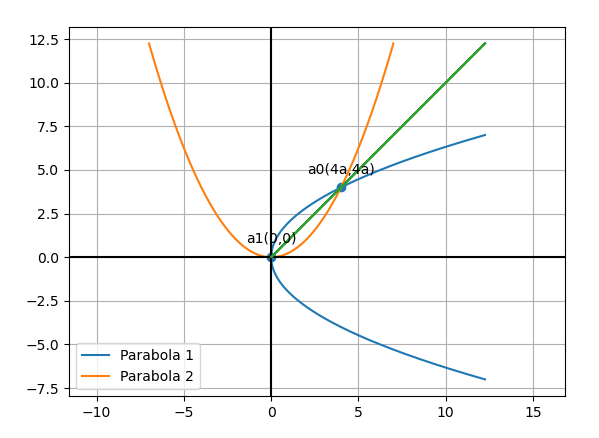
\includegraphics[width=\columnwidth]{con.png}
    \label{fig:my_label}
\end{figure}
\section{\textbf{Solution}}
The given equation of parabola $x^2 = 4ay$ can be written in the general quadratic form as
\begin{align}
    \label{eq:conic_quad_form}
    \vec{x}^{\top}\vec{V}\vec{x}+2\vec{u}^{\top}\vec{x}+f=0
    \end{align}
 
where
\begin{align}
 \label{eq:V_matrix}
 \vec{V} &= \myvec{1 & 0\\0 & 0},
 \\
 \label{eq:u_vector}
 \vec{u} &= \myvec{0\\-2a},
 \\
 \label{eq:f_value}
 f &= 0
 %\\
\end{align}
\\
And also for second Parabola,\\
The given equation of parabola $y^2 = 4ax$ can be written in the general quadratic form as
\begin{align}
    \label{eq:conic_quad_form}
    \vec{x}^{\top}\vec{V}\vec{x}+2\vec{u}^{\top}\vec{x}+f=0
    \end{align}
where
\begin{align}
 \label{eq:V_matrix}
 \vec{V} &= \myvec{0 & 0\\0 & 1},
 \\
 \label{eq:u_vector}
 \vec{u} &= \myvec{-2a\\ 0},
 \\
 \label{eq:f_value}
 f &= 0
 %\\
\end{align}
\\
Since it is given that a line is passing through both the intersection points of these two parabola.\\
So, the equation of that line is $y=x$.\\
The points of intersection of the line 
\begin{align}
 L: \quad \vec{x} = \vec{q} + \mu \vec{m} \quad \mu \in \mathbf{R}
\label{eq:conic_tangent}
\end{align}
with the conic section are given by
\begin{align}
\vec{x}_i = \vec{q} + \mu_i \vec{m}
\label{eq:conic_tangent_pts}
\end{align}
%
where
{\tiny
\begin{multline}
\mu_i = \frac{1}
{
\vec{m}^T\vec{V}\vec{m}
}
\lbrak{-\vec{m}^T\brak{\vec{V}\vec{q}+\vec{u}}}
\\
\pm
\rbrak{\sqrt{
\sbrak{
\vec{m}^T\brak{\vec{V}\vec{q}+\vec{u}}
}^2
-
\brak
{
\vec{q}^T\vec{V}\vec{q} + 2\vec{u}^T\vec{q} +f
}
\brak{\vec{m}^T\vec{V}\vec{m}}
}
}
\end{multline}

From the line y=x the vectors q,m are taken,
\begin{equation}
\vec{q}=\myvec{0\\0}
\end{equation}

\begin{equation}
\vec{m}=\myvec{1\\1}
\end{equation}
\\
\textbf{For Parabola 1},\\

by substituting eq(2),(3),(4),(12),(13) in eq(11)
\begin{equation}
\mu_i=2
\end{equation}

substituting eq(12),(13),(14) in eq(10) ,\\
the intersection points on the parabola are
\begin{equation}
\vec{a_0}=\myvec{4\\4}
\end{equation}
\begin{equation}
\vec{a_1}=\myvec{0\\0}
\end{equation}\\
\textbf{For parabola 2},
by substituting eq(6),(7),(8),(12),(13) in eq(11)
\begin{equation}
\mu_i=2
\end{equation}
substituting eq(12),(13),(17) in eq(10) ,\\
the intersection points on the parabola are
\begin{equation}
\vec{a_0}=\myvec{4\\4}
\end{equation}
\begin{equation}
\vec{a_1}=\myvec{0\\0}
\end{equation}\\
So, Here we can clearly see that the both the Parabolas are intersecting each other at two points i.e \\
at  $\vec{a_0}=\myvec{4a\\4a}$ and $\vec{a_1}=\myvec{0\\0}$
\\
Now,\\
\textbf{Case 1 :}
As the line $ 2bx+3cy+4d = 0$ passes through the intersection points of both parabola ,\\
So, at $\vec{a_1}=\myvec{0\\0}$
\\
$ 2b(0)+3c(0)+4d = 0$ \\
$ \Rightarrow 4d =0 $ \\
Also , $d = 0$\\
\textbf{Case 2 :}
As the line $ 2bx+3cy+4d = 0$ passes through the intersection points of both parabola ,\\
So, at $\vec{a_0}=\myvec{4a\\4a}$
\\
$ 2b(4a)+3c(4a)+4d = 0$ \\
So,\\
$\Rightarrow 8ab+12ac= 0$  (Since d=0)\\
$\Rightarrow 4a(2b+3c) = 0 $\\
Since $ a\neq 0$ \\
we can write ,,\\
$2b+3c=0$\\
Also ,
$ (2b+3c)^2 = 0$ \\
So,\\
we can also say that ,\\
$ d^2 + (2b+3c)^2 = 0$\\
So we can conclude that option D is the correct option




\section{\textbf{Code Link}}

\begin{lstlisting}
https://github.com/aadrshptel/Fwc_module1/tree/main/Assignments/Matrix%20assignments/Conics/codes
\end{lstlisting}
Execute the code by using the command\\
\textbf{python3 conic.py}



\end{document}